\begin{GreyBox}
    \vskip-1cm
    \begin{block}{\GHead{Results}} 
        \begin{center}
            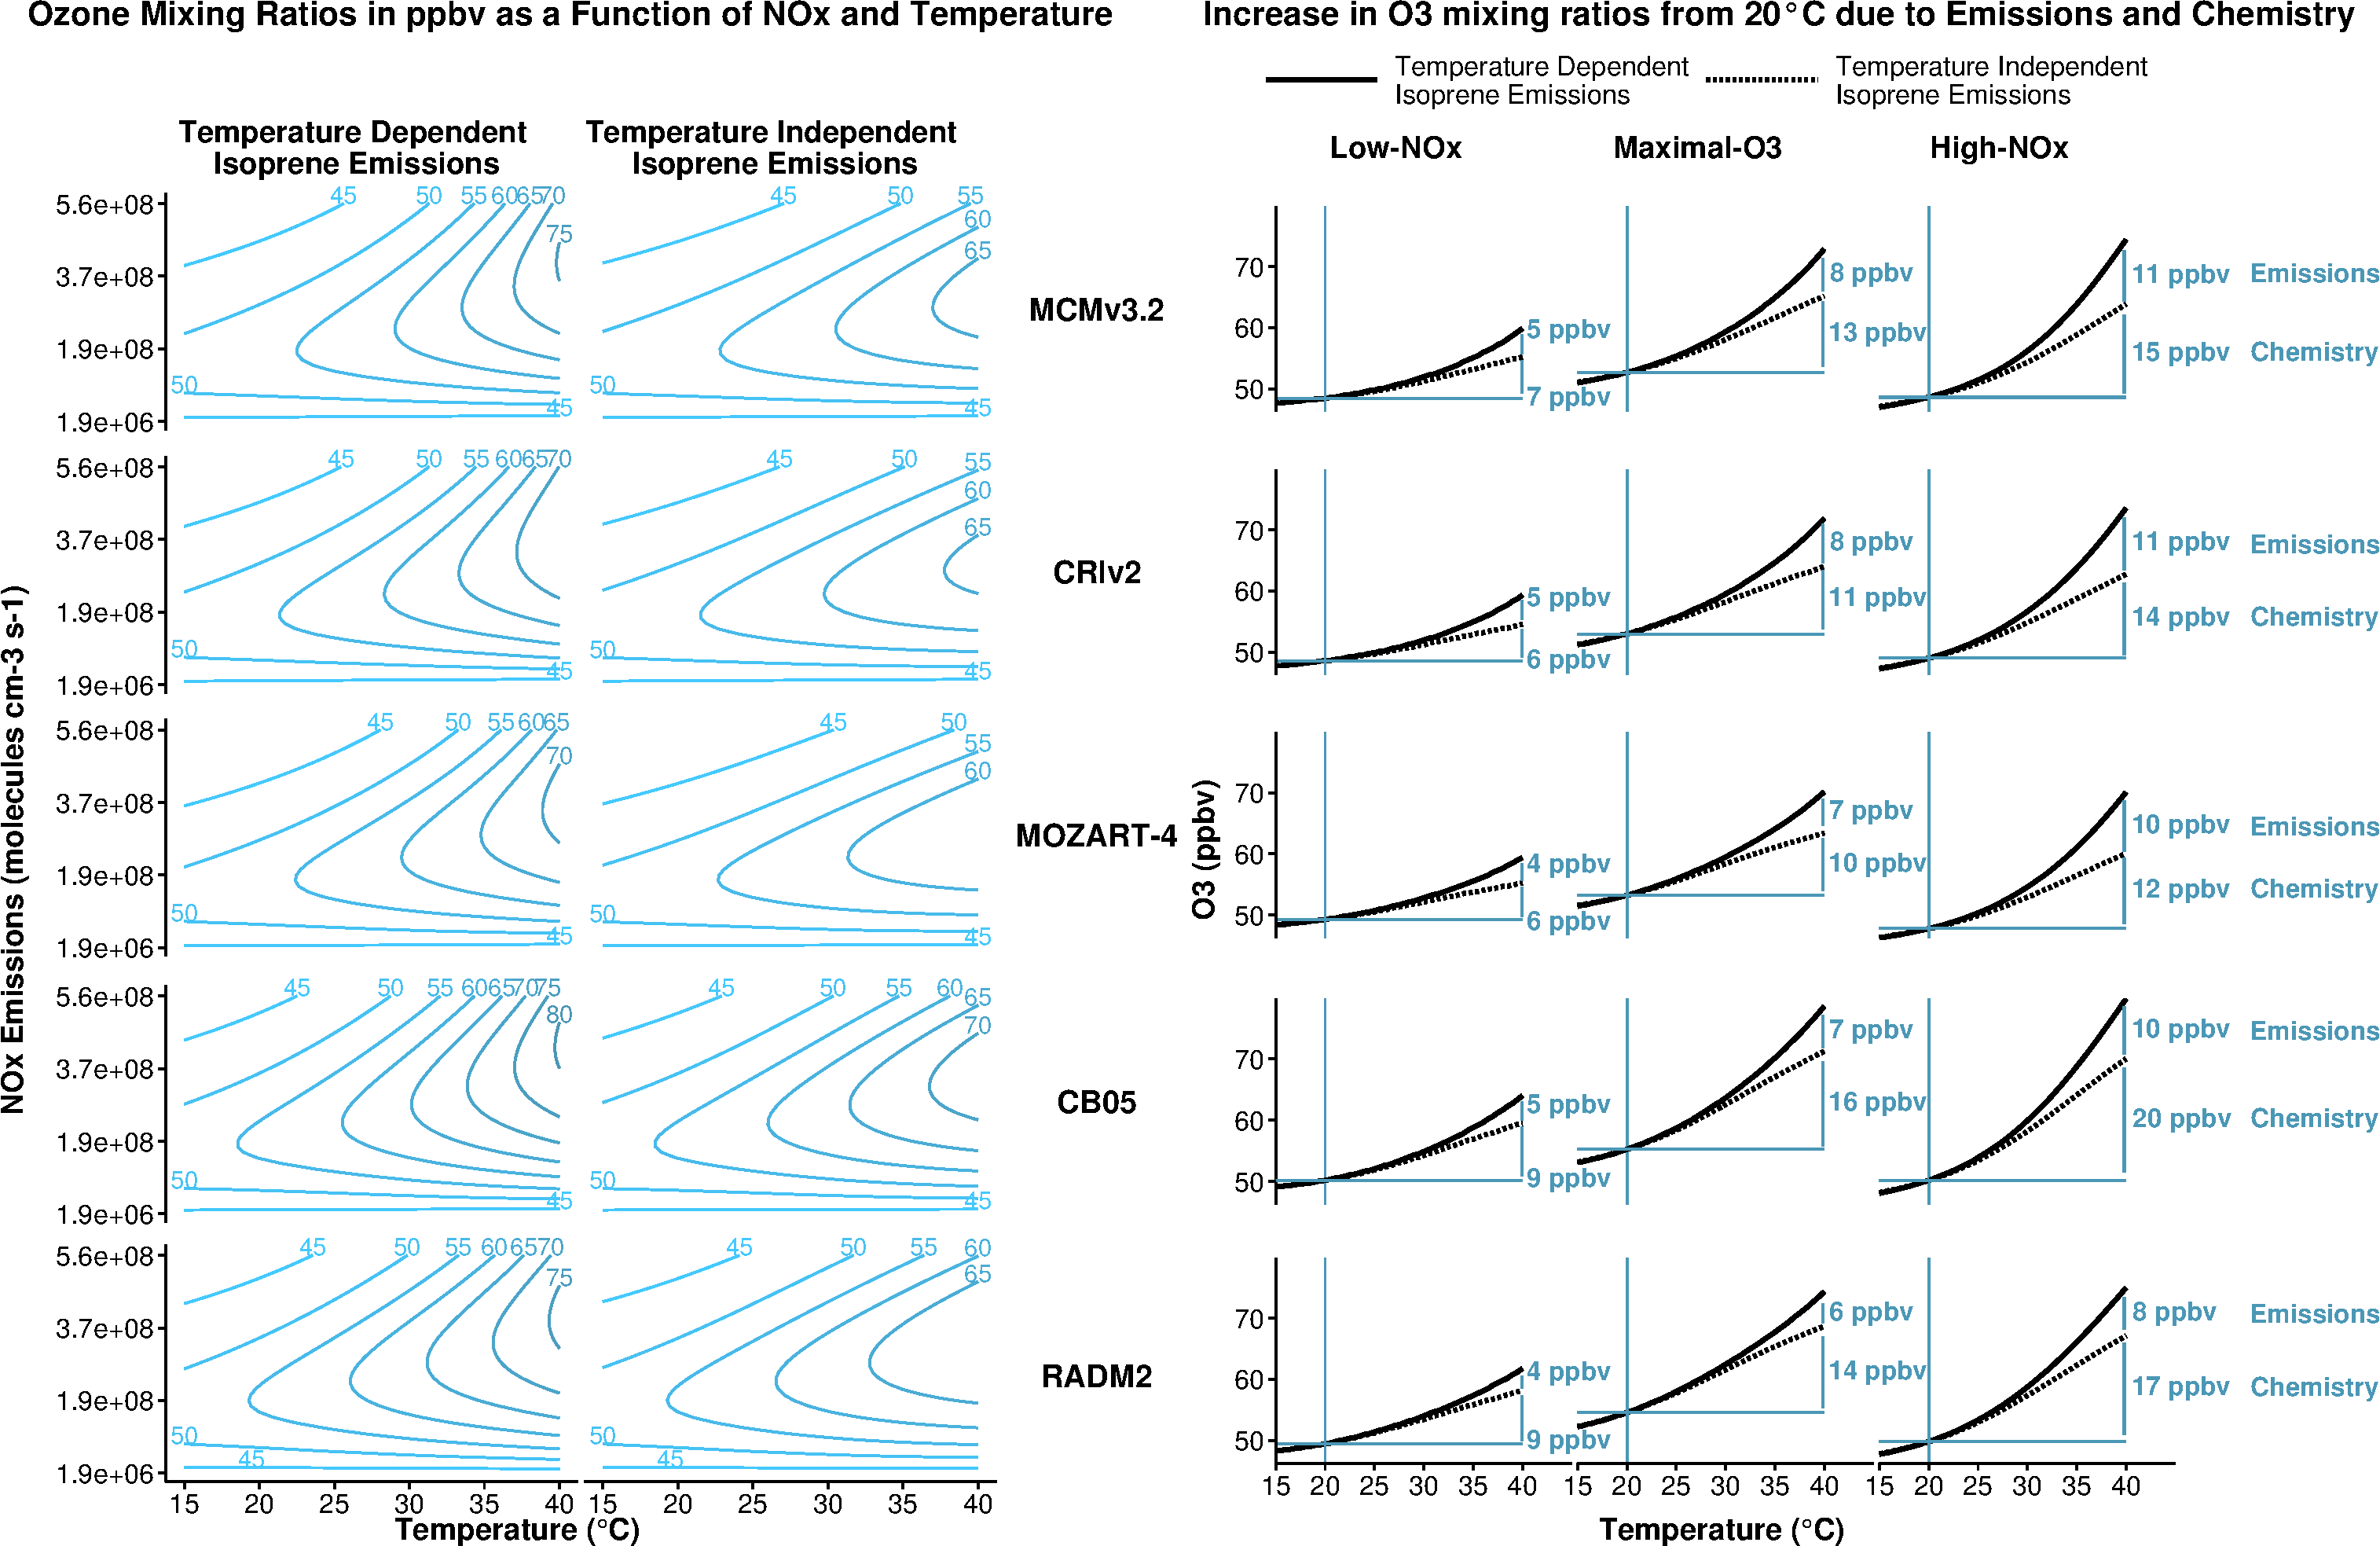
\includegraphics[width = \textwidth]{Plotting/results}
        \end{center}
        \begin{columns}[c]
            \column{0.45\textwidth}
                \begin{WhiteBox}
                    \begin{itemize} \vspace{2mm}
                        \item Highest ozone with temperature dependent source of isoprene and high \ce{NO_x}. \vspace{5mm}
                        \item Lowest ozone with low \ce{NO_x} levels. \vspace{5mm}
                        \item Non-linear relationship of ozone with \ce{NO_x} and temperature reproduced by all chemical mechanisms. \vspace{5mm}
                        \item Highest ozone produced using RADM2 and CB05 chemical mechanisms. \vspace{5mm}
                    \end{itemize}
                \end{WhiteBox}
            \column{0.45\textwidth}
                \begin{WhiteBox} \vspace{2mm}
                    \begin{itemize}
                        \item Largest increases in ozone at $40$~$^{\circ}$C due to increased reaction rates not higher isoprene emissions. \vspace{10mm}
                        \item Largest increases in ozone with high \ce{NO_x} conditions. \vspace{10mm}
                        \item CB05 and RADM2 have lowest increase in ozone due to isoprene emissions but highest increase due to chemistry. \vspace{10mm} 
                    \end{itemize}
                \end{WhiteBox}
        \end{columns}
    \end{block}
\end{GreyBox}
